\documentclass[11pt, oneside]{article}   	% use "amsart" instead of "article" for AMSLaTeX format
\usepackage{geometry}                		% See geometry.pdf to learn the layout options. There are lots.
\geometry{letterpaper}                   		% ... or a4paper or a5paper or ... 
\usepackage{cite}
\usepackage{graphicx}				% Use pdf, png, jpg, or eps§ with pdflatex; use eps in DVI mode
								% TeX will automatically convert eps --> pdf in pdflatex		
\usepackage{amssymb}
\usepackage{url}
\usepackage{titling}
\usepackage[bottom]{footmisc}


\title{The Oncoming Death of Metaphor}
\author{Andrew Kowalczyk}
\date{October 31, 2013}							% Activate to display a given date or no date

\begin{document}
\maketitle
\centerline{\textbf{Abstract}}
Metaphor, in the broadest sense of the term for the discipline of a computer science, is a group of user interface images and activities that take advantage of particular proficiencies that users already have of other domains. Typical examples include using a tool or some kind of gear to represent Settings or Preferences on some operating system or ``flipping'' a page by swiping on a touch interface in a book reading app. Although metaphor is extremely useful and even though the majority of people designing user interfaces currently employ it heavily, I argue that the beginning of the end of metaphor is on its way and should be sought out after.

\pagebreak
\section{Metaphor and the Human Brain} 
My grandmother was a pharmacist at an army hospital in Warsaw, Poland for 50 years up until her retirement. She used paper and pen for everything related to her job: logging the number of milligrams of drugs taken out to make antibacterial creams, logging the number of liters of isopropyl alcohol given to surgeons for disinfecting, filling out prescriptions, etc. On a not so fateful day, her management let her know that they would be switching from paper and pen to a machine running Windows XP for all her work related logging. A once incredibly fast and efficient pharmacist was rendered helpless by a technology that was meant to streamline her work. She eventually learned how to work on that machine after countless hours at work asking her younger coworkers for guidance. I still see her struggling with her laptop at home when I Skype with her. \footnote{Yes, my 83 year old grandmother knows how to use Skype, and I am incredibly proud.}

Before the invention of the modern personal computer, imagine (or recall if you can) what seeing one for the first time would be like.
Personally, I clearly remember seeing a large bundle sitting on my father's desk. It consisted of a system unit, with a magnetic spinning hard drive, a floppy drive slot, a CRT monitor that allowed you to degauss with the press of a button (which was more interesting than any program installed on that machine), a mouse with an actual rolling ball inside, and a keyboard that could wake up a whole house on Christmas Eve. My best guess was that it was a typewriter and television put together that hummed a bit too loud for my liking.

If you were to ask random people what they know about the brain, more often than not, most of them would mention something along the lines that the brain has two hemispheres, and that the left side is perceived as being analytical, technical, and logical and that the right is perceived as being creative, artistic, and expressive. Although this separation in the brain has been proven to not be so dichotomic by studies and research, it provides an interesting parallel to computer scientists and their employment of metaphor.

Just as the corpus calossum, the flat bundle of neural fibers beneath the cortex, connects the left and right cerebral hemispheres and facilitates interhemispheric communication, metaphor is the connection between the highly artistic and expressive people and the highly  technical and analytical people in this world. Or put more simply, metaphor is the connection between computer scientists and the nontechnical people. My grandmother and my younger self represent the kind of people that metaphor aims to assist in learning new technologies. How else is 65 year old woman or an eight year old child supposed to learn how to interact with a graphical user interface when they have never tried one?

The amount people that have not used a graphical user interface has extremely diminished since the day that Windows XP machine came rattling into my grandmother's pharmacy. It is clear that more and more people are using computers. The rates in which computer use has increased in homes in the United States is staggering. From the year of 1984 to 2010, the percentage of households with a computer went from 8.2\% to 76.7\%. Within little than over a fourth of a decade, that percentage roughly saw a 835\% increase. \cite{computer-use} \footnote{See Figure at the back of the paper}
One can assume that since there are more computers in the homes of Americans, there are more people in America that use them. Or in other words, America has a lot more technologically apt people simply due to their exposure to a computer. Due to the margin of people who have a computer and know how to use one expanding, this shows that the target audience for any technology should be geared towards people who are slightly technologically apt.

\section{A history of Metaphor}

Metaphor may seem like a new phenomenon in CS (Computer Science) to people not involved in the field. Yet, metaphor has been a topic of conversation since even before GUI's (graphical user interfaces) came to stardom.

It has always been the topic of many discussions and the focus of countless debates.
In years like 1998, writers like Faulkner were writing that, ``Designers of systems should, where possible, use metaphors that the user will be familiar with.'' \cite{essence}  Or in 1995, Hill wrote, ``Metaphors make it easy to learn about unfamiliar objects.'' \cite{practical} Or even earlier in 1992, Macintosh's human interface guidelines say, ``Use metaphors involving concrete, familiar ideas and make the metaphors plain, so that users have a set of expectations to apply to computer environments.'' \cite{apple}

Wait, wait, wait. Did you read all that? Every single one of the citations mentioned that metaphors should be used in design. Every single one. And for a good reason.


\cite{reification}
say why metaphor is awesome

\cite{bae16}

\section{Case study: Apple's push away from metaphor}
Apple has realized that as technology is becoming more and more ingrained into our society, the aid of metaphor is largely shrinking. With their new releases of iOS 7 and OSX 10.9 Mavericks, Apple commenced their push away from metaphor.

\subsection{iOS7}
With no surprise, the release of iOS 7 garnered much support and much backlash. Many of the large criticisms include its transition to overly simple menus, its change from icons to words, and its unlifelike apps. With it's goal being simplicity, Apple comments on their shift, ``The interface is purposely unobtrusive. Conspicuous ornamentation has been stripped away. Unnecessary bars and buttons have been removed.'' \cite{apple-design} They have realized that \textit{skeuomorhpism}, the design concept of making items represented resemble their real-world counterparts (the definition is surprisingly not too far off from metaphor), serves no purpose in their new operating system.

In the Ars Technica Review of iOS 7, the author Andrew Cunningham isn't afraid to make fun of the previous operating system by mentioning,``Will people understand what the Newsstand folder is for if we don?t make it look like a little wooden shelf? Will people understand that things have been deleted from Passbook if we don?t throw their virtual coupons into a virtual paper shredder?'' \cite{ars-technica-iOS7} These are questions that now sound funny, but as the modern personal computer was being pioneered, these questions would have sounded appropriate.

\subsection{OSX 10.9 Mavericks}
Apple's most recent update of the big cat operating system line followed iOS7 in its push away from metaphor the most part, yet not entirely. It dealt away with most lifelike textures like leather, linen, etc. I turn to John Siracusa, famous for his in-depth articles about Mac operating systems.

A prime example of why Apple went for a \textit{flatter} and less realistic look is the Address Book application, introduced in OSX 10.7 Lion, which is now renamed as Contacts in 10.9. Siracusa's main criticisms of Contacts include that it is ``boring'' and that it removed ``beauty'' and ``fun''.  \cite{ars-technica-mavericks} That's really about it. He says it wouldn't stand out in a crowd. The overall change in the application can be summarized as so, ``Apple took the Mountain Lion versions, removed the graphical frills, and updated the UI enough to work correctly without them.'' \cite{ars-technica-mavericks} 

His review for the Address Book application in Lion had some actual criticisms beyond the application's design. The old app looked like a book: leather-bound and it even had a red ribbon bookmark. But, the app did not behave like a book. The pages can't be turned, the bookmark can't be removed, groups were located on a different page (you can't look at three pages at once in a book), \cite{ars-technica-lion} The application has ``mixed [metaphors] that sends mixed signals.''  The applications, like Address Book and iCal (another prime example employing skeuomorphism), were simply limited by their physical counterparts and implied functionality that simply doesn't exist. \cite{ars-technica-lion}

Siracusa held a generally negative review about the updated Contacts application in Mavericks. Yet for Address Book, he mentioned serious issues with the applications usability due to its heavy employment of metaphor. This is the the actual problem. Apple loves beauty, but has realized that usability trumps aesthetics. Siracusa mentions his opinion of usability vs. aesthetics in his Lion review as he says, ``People will take "really cool-looking but slightly harder to use" over "usable but ugly" any day.'' Yet, if one explores a little further into his review, he mentions, ``We're far past the point where computer interfaces need to reference their forebearers in the physical world in order to be understandable.'' The user interface's usability should be the top priority, not the way it looks. \footnote{See Figures ~\ref{fig:address-book} and ~\ref{fig:contacts} at the end of the paper to see a visual comparison of Address Book and Contacts.}
 
\subsection{Summary}
Apple realizes the potential of \textit{easing the brakes} on metaphor and skeuomorphism. They understand that their users are, god forbid, \textit{smart} enough to learn new ways of interacting with applications.


\section{Djikstra's argument against metaphor}
Edsgar Dijkstra, one of the most important computer scientists, claimed that metaphor was extremely damaging to the profession even before the age of personal computers and the rise of GUI's. In a transcript titled \textit{On the cruelty of really teaching computing science}, he initially introduces his argument by explaining the way in which we approach tomorrow's struggles. He says the most common way of facing tomorrow is by ``means of metaphors and analogies'' so that ``we try to link the new to the old, the novel to the familiar''. He makes the claim that coping with "radical novelties" in this fashion is extremely detrimental for the field of computer science for a number of reasons.

First, he does admit that in the cases of ``sufficiently slow and gradual change'', metaphor works reasonably well. A powerful example of this is the field of mathematics. The community of this discipline has never really challenged the ways of teaching, learning, and understanding itself. Djikstra puts it the best, ``Simply by definition, mathematics will continue to be what it used to be.''

Yet, in cases of ``sharp discontinuity'', the employment of metaphor breaks down. Metaphor becomes more ``misleading than illuminating''. It makes sense, doesn't it? In a field that changes nearly daily, the heavy reliance of our past limits the way in which the field can evolve.
\cite{ewd1036}

\section{Why and where metaphor works}
\subsection{Why}
Before looking at where and why metaphor doesn't work, let us explore where and why it does. Let us turn to Ben Shniederman, Norman Nielsen, and Bruce Tognazinni. Each of these very influential people have their own lists or rules for usability within a user interface. I could write about why these people are qualified to make such lists or rules, but in due time, you might just have to trust me and do some reading on your own about these fascinating people. 

Within Shniederman's Eight Golden Rules, Nielsen's Ten Usability Heuristics, and Tognazzini's Sixteen First Principles of Interaction Design, there is a unifying rule.

\cite{shniederman-golden-rules} \cite{tognazzini-first-principles} \cite{nielsen-usability-heuristics}

Tognazzini actually explicitly states metaphor and their use as one of his sixteen first principles of design.

Of all of their rules, there is a unifying one. The most important are to offer simple error handling. 

Of the rules mentioned by Shniederman, metaphor is relevant to striving for consistency and to prevent errors. If a user is exposed to the same type of metaphors in a user interface, they are more likely to encounter less errors during their experience. This metaphor can be helped 


\subsection{Where}
Let us also look to Norman

\section{Why and where metaphor doesn't work}

\subsection{Why}
\subsection{Where}


\section{Conclusion}
Metaphor's usefulness has been, without contest, one of the most important factors in the way in which humans interact with computers. Yet, metaphor is slowly becoming less and less useful in today's world for a few reasons:
\begin{enumerate}
\item With a generation that has literally grown up with technology, metaphor is less and less needed because these users are becoming more and more technologically apt.
\item Relying on the past in a field that changes and expands frequently limits designers because it gives less freedom to employ their creativity and it limits users because it disallows for true learning.
\end{enumerate}
Due to these reasons, the employment of metaphor should be 

\pagebreak
\bibliography{death-of-metaphor}
\bibliographystyle{plain}

\pagebreak
\textbf{\Large{Figures}}
\begin{figure}[!ht]
\begin{center}
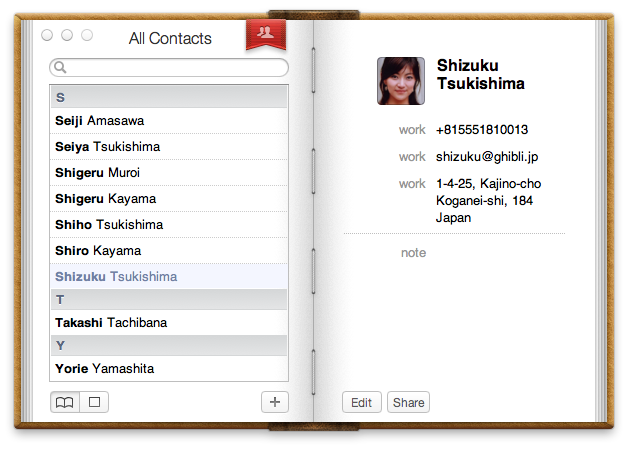
\includegraphics[height=8cm]{address-book.png}
\caption{\label{fig:address-book} Address Book in OSX 10.7 Lion}
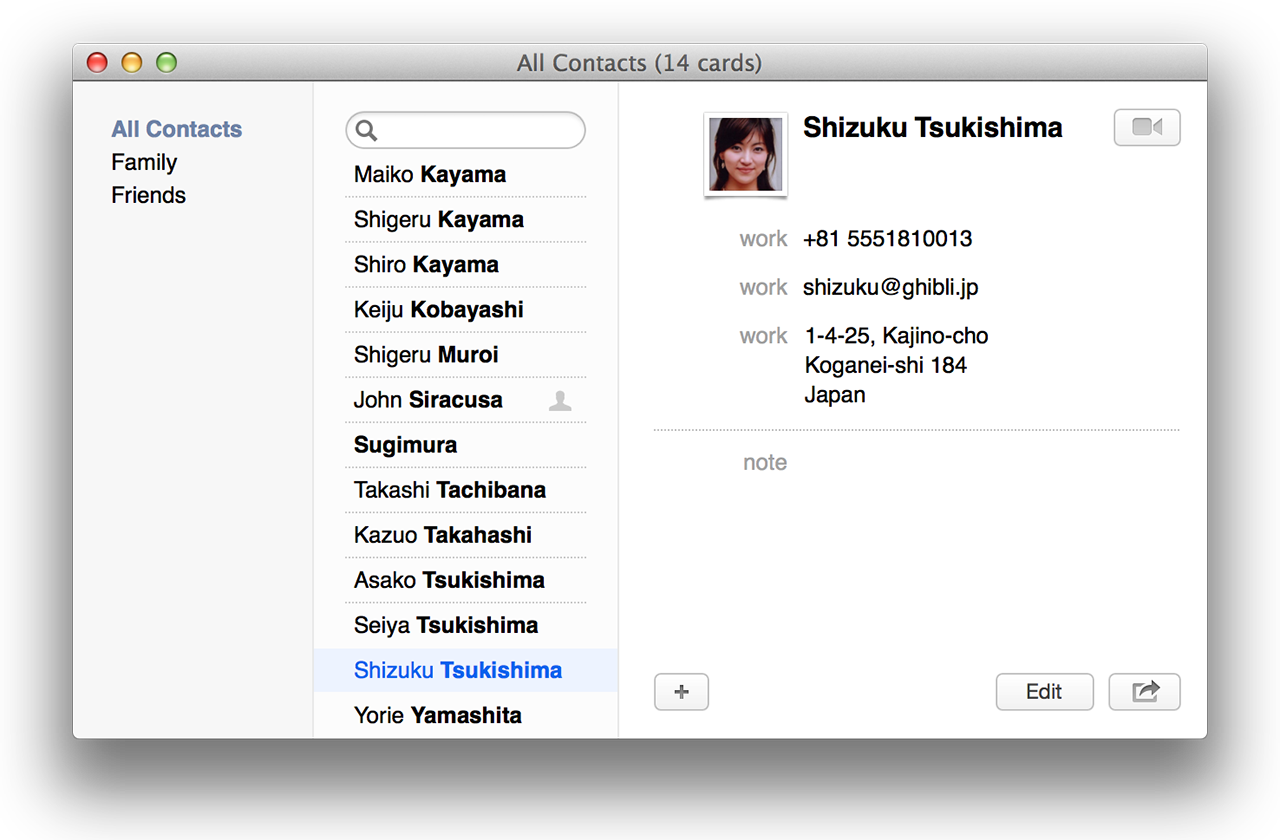
\includegraphics[height=8cm]{contacts.png}
\caption{\label{fig:contacts} Contacts in OSX 10.9 Mavericks}
\end{center}
\end{figure}


\end{document}  	